\chapter{ANALISIS ASOSIASI TEMPORAL}
\label{chap:temporal}\label{sec:hasil-e}
% Bagian E: analisis asosiasi temporal (Mahesa, notebook 07_temporal).
Bab ini membandingkan pola asosiasi konferensi pada empat periode, yaitu 2015--2017, 2018--2020, 2021--2023, dan 2024--2025, menggunakan \textit{author-year-based database} (Bab~\ref{sec:hasil-t3}). Setiap periode diperlakukan sebagai \textit{database} tersendiri: transaksinya adalah pasangan (penulis, tahun) pada periode itu, dan penyebut \textit{support} adalah seluruh transaksi periode tersebut. \textit{Mining} memakai FP-Growth \cite{han2000} yang sudah divalidasi pada Subbab~\ref{sec:hasil-t4-fp-validasi}, dan \textit{rules} dibangkitkan dengan \textit{min\_conf} 50\% seperti \textit{Task} 5.

\section{Data per periode dan pemilihan \textit{min\_sup}}
\label{sec:hasil-e-data}
Tabel~\ref{tab:e-periode} menunjukkan keempat periode memiliki ukuran yang sebanding dan porsi transaksi berisi minimal dua konferensi yang mirip. Periode 2024--2025 hanya dua tahun dan data 2025 belum lengkap, tetapi karena \textit{support} dihitung relatif terhadap jumlah transaksi periode itu sendiri, perbedaan ukuran tidak langsung mengubah \textit{support}.

\begin{table}[ht]
\caption{Transaksi dan jumlah \textit{rules} per periode}
\label{tab:e-periode}
\small
\begin{tabular}{@{}lrrrrrr@{}}
\toprule
 & & & & \multicolumn{3}{c}{\textbf{\textit{Rules} pada \textit{min\_sup}}} \\
\cmidrule(lr){5-7}
\textbf{Periode} & \textbf{Transaksi} & \textbf{$\geq$ 2 konf.} & \textbf{$\geq$ 20 konf.} & \textbf{0,01\%} & \textbf{0,02\%} & \textbf{0,05\%} \\
\midrule
2015--2017 & 922.051 & 29,2\% & 137 & 70 & 17 & 2 \\
2018--2020 & 1.080.824 & 28,2\% & 272 & 130 & 32 & 4 \\
2021--2023 & 1.195.907 & 28,1\% & 511 & 480 & 113 & 25 \\
2024--2025 & 886.812 & 30,8\% & 582 & 7.741 & 1.874 & 282 \\
\bottomrule
\end{tabular}
\end{table}

\textit{Min\_sup} yang dipakai pada \textit{Task} 4 terlalu tinggi untuk \textit{database} ini. Sebanyak 71\% transaksi \textit{author-year} hanya berisi satu konferensi, sehingga pada \textit{min\_sup} 0,1\% tiga periode pertama hanya menghasilkan 1, 0, dan 3 \textit{rules}. Karena itu dipakai tiga ambang yang lebih rendah, yaitu 0,01\%, 0,02\%, dan 0,05\%. Ketiganya dijalankan, lalu satu ambang dipilih sebagai ambang utama dengan kriteria yang ditetapkan sebelum melihat polanya: setiap periode harus memiliki minimal 15 \textit{rules}, dan minimal 80\% \textit{rules} setiap periode harus lolos uji ketahanan.

Uji ketahanan mengulang \textit{mining} setelah transaksi berisi 20 konferensi atau lebih dalam satu tahun dikosongkan, dengan penyebut tetap. Transaksi seperti ini sebagian besar berasal dari nama umum yang menggabungkan beberapa orang (Subbab~\ref{sec:hasil-statistik-tx}). Tabel~\ref{tab:e-tahan} menunjukkan porsi \textit{rules} yang tetap ditemukan.

\begin{table}[ht]
\caption{Porsi \textit{rules} yang tetap ditemukan tanpa transaksi berisi 20 konferensi atau lebih}
\label{tab:e-tahan}
\small
\begin{tabular}{@{}lrrrr@{}}
\toprule
\textbf{\textit{min\_sup}} & \textbf{2015--2017} & \textbf{2018--2020} & \textbf{2021--2023} & \textbf{2024--2025} \\
\midrule
0,01\% & 96\% & 100\% & 93\% & 64\% \\
0,02\% & 94\% & 100\% & 98\% & 67\% \\
0,05\% & 100\% & 100\% & 96\% & 78\% \\
\bottomrule
\end{tabular}
\end{table}

Tidak ada ambang yang memenuhi kedua kriteria karena periode 2024--2025 selalu di bawah 80\%. Ambang 0,05\% juga tidak memenuhi syarat jumlah \textit{rules} (2 dan 4 \textit{rules} pada dua periode awal). Karena tanpa \textit{rules} tidak ada yang dapat dibandingkan, jumlah \textit{rules} tetap dijadikan syarat, dan di antara ambang yang memenuhinya dipilih ketahanan terbaik, yaitu \textbf{0,02\%}. Pada tiga periode pertama ketahanannya 94\% sampai 100\%, sehingga hanya \textit{rules} 2024--2025 yang perlu dibaca hati-hati.

\section{\textit{Frequent itemsets} per periode}
\label{sec:hasil-e-fpm}
Pada 0,02\%, jumlah \textit{itemset} berisi dua konferensi atau lebih adalah 279, 376, 662, dan 2.380 dari periode pertama sampai terakhir, dan \textit{itemset} berisi empat konferensi atau lebih naik dari 1 menjadi 710. Sebaliknya, jumlah konferensi tunggal yang \textit{frequent} turun dari 1.600 menjadi 1.266, padahal ambang \textit{count} 2024--2025 paling rendah (178 transaksi). Penulis makin terkumpul pada konferensi yang sama, dan konferensi itu makin sering muncul bersama dalam satu tahun.

Tabel~\ref{tab:e-pasangan} menunjukkan lima pasangan teratas setiap periode. Pada 2015--2017, pasangan teratas tersebar di telekomunikasi, kendali, robotika, dan komunikasi optik. Hanya satu dari sepuluh pasangan teratas periode ini (AAAI + IJCAI) yang memuat AAAI, NeurIPS, ICML, ICLR, ACL, atau EMNLP. Pada 2024--2025, sembilan dari sepuluh pasangan teratas memuat salah satu konferensi itu, dan pengecualiannya hanya CVPR + ICCV. \textit{Support} ICLR + NeurIPS naik dari 0,18\% pada 2018--2020 menjadi 1,04\%, sedangkan GLOBECOM + ICC turun dari peringkat pertama ke luar sepuluh besar.

\begin{table}[ht]
\caption{Lima pasangan konferensi dengan \textit{support} tertinggi per periode (\textit{min\_sup} 0,02\%)}
\label{tab:e-pasangan}
\footnotesize
\setlength{\tabcolsep}{4pt}
\begin{tabular}{@{}rllll@{}}
\toprule
\textbf{\#} & \textbf{2015--2017} & \textbf{2018--2020} & \textbf{2021--2023} & \textbf{2024--2025} \\
\midrule
1 & GLOBECOM + ICC & CVPR + ECCV & ICML + NeurIPS & ICLR + NeurIPS \\
2 & ACC + CDC & GLOBECOM + ICC & ACL + EMNLP & ICML + NeurIPS \\
3 & ICRA + IROS & ICML + NeurIPS & CVPR + ICCV & CVPR + NeurIPS \\
4 & ECOC + OFC & ICRA + IROS & ICLR + NeurIPS & ACL + EMNLP \\
5 & GLOBECOM + VTC Fall & AAAI + IJCAI & CVPR + NeurIPS & ICLR + ICML \\
\bottomrule
\end{tabular}
\end{table}

\section{\textit{Association rules} per periode}
\label{sec:hasil-e-rules}
Jumlah \textit{rules} naik tajam menuju 2024--2025 pada ketiga ambang (Tabel~\ref{tab:e-periode} dan Gambar~\ref{fig:e-rules}). Median \textit{lift} pada 0,02\% turun dari 49,1 dan 49,2 menjadi 28,0 dan 20,2. \textit{Rules} baru berpusat pada konferensi besar, dan seperti pada Subbab~\ref{sec:hasil-t5-lift}, \textit{rule} yang menuju konferensi besar memiliki \textit{lift} lebih rendah. \textit{Rule} satu-ke-satu hampir tidak ada (2, 1, 1, dan 0): dalam satu tahun, menerbitkan di satu konferensi jarang cukup untuk memprediksi konferensi lain dengan \textit{confidence} 50\%.

\begin{figure}[ht]
\centering
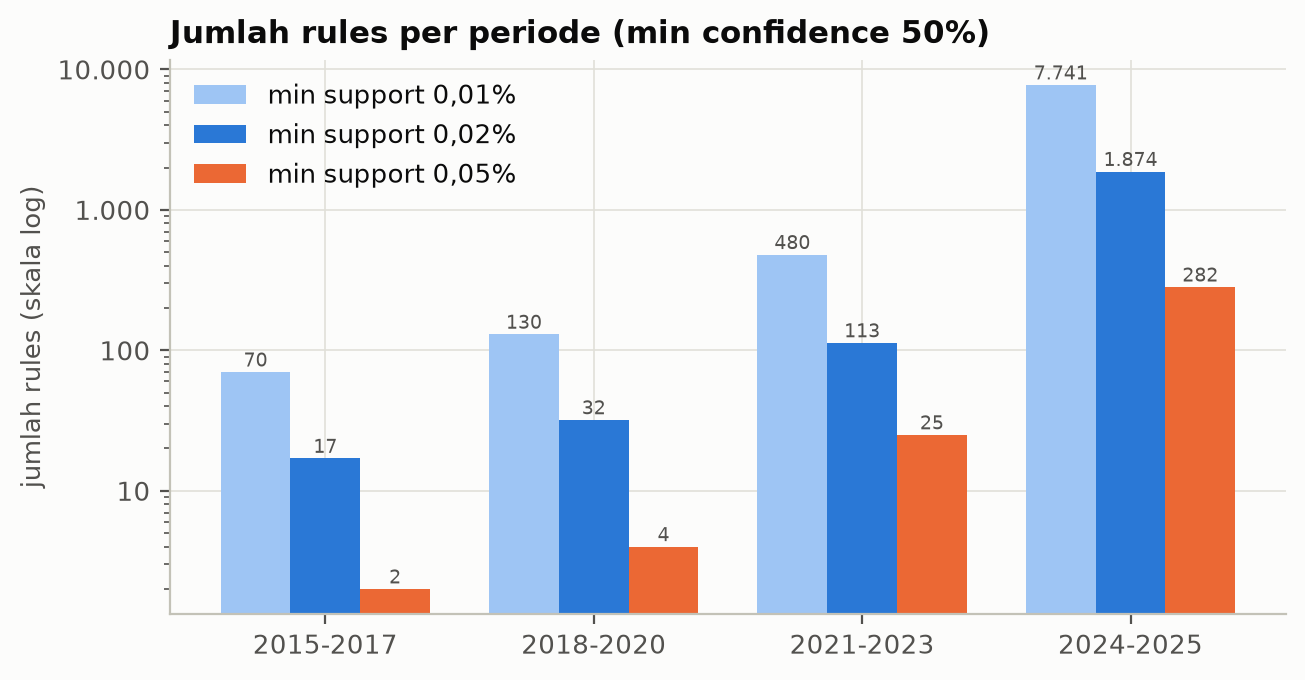
\includegraphics[width=0.9\textwidth]{images/hasil/t7_rules_per_periode.png}
\caption{Jumlah \textit{rules} per periode pada tiga \textit{min\_sup} (skala log, \textit{min\_conf} 50\%)}
\label{fig:e-rules}
\end{figure}

Sepuluh \textit{lift} tertinggi 2015--2017 tersebar di banyak kelompok, misalnya AISTATS + ICML $\Rightarrow$ NeurIPS (\textit{lift} 113,8), ASRU + ICASSP $\Rightarrow$ INTERSPEECH (104,9), dan ACC + ECC $\Rightarrow$ CDC (68,0). Pada 2024--2025, seluruh sepuluh \textit{lift} tertinggi adalah \textit{rule} tiga atau empat konferensi menuju dua konferensi yang memuat ACL atau EMNLP bersama ICLR atau ICML, misalnya EMNLP + ICLR + ACM Multimedia + NeurIPS $\Rightarrow$ ACL + ICML (\textit{lift} 161,9). \textit{Count}-nya hanya 184 sampai 279 transaksi, dan hanya empat dari sepuluh yang lolos uji ketahanan.

\section{Perbandingan \textit{rules} antarperiode}
\label{sec:hasil-e-banding}
Setiap \textit{rule} pada 0,02\% diberi kategori menurut kemunculannya: \textit{bertahan} (lolos di keempat periode), \textit{muncul} (tidak lolos di awal, lalu lolos terus sampai 2024--2025), \textit{hilang} (lolos di awal, lalu tidak lolos sampai 2024--2025), dan \textit{berselang} (pola lain). \textit{Support}, \textit{confidence}, dan \textit{lift} setiap \textit{rule} juga dihitung langsung dari transaksi di setiap periode, termasuk periode saat \textit{rule} itu tidak lolos.

\begin{table}[ht]
\caption{Jumlah \textit{rules} per kategori pada tiga \textit{min\_sup}}
\label{tab:e-kategori}
\small
\begin{tabular}{@{}lrrr@{}}
\toprule
\textbf{Kategori} & \textbf{0,01\%} & \textbf{0,02\% (utama)} & \textbf{0,05\%} \\
\midrule
Bertahan & 13 & 1 & 0 \\
Hilang & 39 & 11 & 2 \\
Berselang & 113 & 27 & 7 \\
Muncul & 7.704 & 1.865 & 281 \\
\bottomrule
\end{tabular}
\end{table}

Tabel~\ref{tab:e-kategori} menunjukkan gambaran yang sama pada ketiga ambang: 97\% sampai 98\% \textit{rules} adalah \textit{rules} yang muncul, dan \textit{rules} yang bertahan sangat sedikit. Jumlah pasti \textit{rules} bertahan bergantung pada ambang (13, 1, dan 0), sehingga yang disimpulkan adalah polanya, bukan angkanya.

\textbf{\textit{Rule} yang bertahan.} Pada 0,02\%, satu-satunya \textit{rule} yang bertahan adalah AISTATS + ICML $\Rightarrow$ NeurIPS. \textit{Confidence}-nya hampir tetap (60\%, 61\%, 61\%, dan 58\%), sedangkan \textit{count}-nya naik dari 204 menjadi 716 pada 2021--2023.

\textbf{\textit{Rules} yang hilang.} Sebelas \textit{rules} hilang, tujuh di antaranya melibatkan GLOBECOM dan ICC. Tabel~\ref{tab:e-hilang} menunjukkan bahwa hilangnya bukan karena hubungan berhenti. Ada tiga penyebab:
\begin{enumerate}
\item \textbf{Data tidak tercatat.} DBLP tidak mencatat ICCC pada 2024--2025, sehingga dua \textit{rule} ICCC hilang karena data. ECOC juga tidak tercatat pada 2016, 2019, dan 2022--2024, dan ICTON tidak tercatat pada 2021--2022.
\item \textbf{\textit{Count} tetap, \textit{database} bertambah.} \textit{Count} \textit{rules} GLOBECOM/ICC relatif datar, sedangkan ambang \textit{count} naik dari 185 menjadi 240 pada 2021--2023 karena jumlah transaksi bertambah. Kombinasinya tidak menghilang, tetapi porsinya mengecil.
\item \textbf{\textit{Confidence} di sekitar 50\%.} Setelah tidak lolos, \textit{confidence} \textit{rules} ini tetap 40\% sampai 64\%, sehingga lolos atau tidaknya ditentukan selisih kecil.
\end{enumerate}
Hanya ACC + ECC $\Rightarrow$ CDC yang \textit{count}-nya juga turun secara absolut (dari 259 menjadi 140).

\begin{table}[ht]
\caption{Beberapa \textit{rule} yang hilang (\textit{min\_sup} 0,02\%; ambang \textit{count} 185, 217, 240, 178)}
\label{tab:e-hilang}
\footnotesize
\setlength{\tabcolsep}{4pt}
\begin{tabular}{@{}lll@{}}
\toprule
\textbf{\textit{Rule}} & \textbf{\textit{Count} per periode} & \textbf{\textit{Confidence} per periode} \\
\midrule
ICC + ICCC $\Rightarrow$ GLOBECOM & 210 / 256 / 325 / 0 & 56\% / 58\% / 59\% / -- \\
GLOBECOM + WCNC $\Rightarrow$ ICC & 475 / 521 / 496 / 533 & 52\% / 48\% / 50\% / 46\% \\
GLOBECOM + SPAWC $\Rightarrow$ ICC & 236 / 194 / 203 / 158 & 63\% / 49\% / 59\% / 54\% \\
ECOC $\Rightarrow$ OFC & 1.721 / 1.558 / 600 / 1.180 & 52\% / 47\% / 48\% / 44\% \\
ASRU $\Rightarrow$ INTERSPEECH & 363 / 221 / 619 / 409 & 50\% / 44\% / 44\% / 47\% \\
ACC + ECC $\Rightarrow$ CDC & 259 / 276 / 170 / 140 & 56\% / 54\% / 49\% / 51\% \\
\bottomrule
\end{tabular}
\end{table}

\textbf{\textit{Rules} yang berselang.} Sebanyak 15 dari 27 \textit{rules} berselang memuat konferensi yang tidak tercatat setiap tahun. Pada DBLP, ICCV hanya tercatat pada tahun ganjil dan ECCV pada tahun genap, sehingga 2015--2017 dan 2021--2023 memiliki dua edisi ICCV, sedangkan 2018--2020 memiliki dua edisi ECCV. Keenam \textit{rule} ICCV hanya lolos pada 2021--2023, dan tiga \textit{rule} ACCV/BMVC dengan ECCV hanya lolos pada 2018--2020. SLT, Odyssey, dan COLING menunjukkan pola yang sama. Pada \textit{author-year-based database}, konferensi seperti ini hanya dapat berpasangan pada tahun penyelenggaraannya, sehingga perbedaan antarperiode untuk konferensi ini terutama mencerminkan jadwal, bukan perubahan minat penulis. Dua belas \textit{rules} sisanya memiliki edisi lengkap di setiap periode dan berselang karena \textit{support} atau \textit{confidence}-nya berada di sekitar ambang.

\textbf{\textit{Rules} yang muncul.} NeurIPS terlibat pada 67\% dari 1.865 \textit{rules} yang muncul, diikuti ICLR (47\%), ACL (45\%), AAAI (43\%), EMNLP (42\%), ICML (40\%), dan CVPR (35\%). Sebanyak 95 \textit{rules} sudah muncul sejak 2018--2020 atau 2021--2023 dan bertahan sampai 2024--2025, dan 94\% sampai 95\% di antaranya lolos uji ketahanan. Sisanya, 1.770 \textit{rules}, hanya ada pada 2024--2025, dan hanya 65\% yang lolos uji ketahanan.

\section{Jawaban pertanyaan Bagian E}
\label{sec:jawab-e}
\textbf{\textit{Frequent itemsets} dan \textit{rules} per periode.} FP-Growth dijalankan pada empat periode dan tiga \textit{min\_sup}. Pada \textit{min\_sup} utama 0,02\%, \textit{itemset} berisi dua konferensi atau lebih berjumlah 279, 376, 662, dan 2.380, dan \textit{rules} berjumlah 17, 32, 113, dan 1.874.

\textbf{Perbandingan dan pola yang bertahan atau berubah.} Hampir seluruh \textit{rules} (98\%) adalah \textit{rules} baru, dan hanya AISTATS + ICML $\Rightarrow$ NeurIPS yang bertahan di keempat periode. \textit{Rules} yang hilang, terutama GLOBECOM/ICC, sebagian besar hanya turun sedikit di bawah ambang karena \textit{count}-nya tetap saat \textit{database} bertambah, atau hilang karena konferensinya tidak tercatat. Lebih dari separuh \textit{rules} yang berselang mengikuti jadwal konferensi yang tidak tahunan.

\textbf{Kemungkinan perubahan tren publikasi.} Pertama, kombinasi konferensi dalam satu tahun makin terpusat pada NeurIPS, ICLR, ICML, ACL, EMNLP, AAAI, dan CVPR. Ini sejalan dengan Subbab~\ref{sec:hasil-tren}, tempat konferensi yang sama tumbuh paling cepat dan porsi sepuluh konferensi teratas naik dari 7,0\% menjadi 11,7\%. Kedua, penulis di konferensi-konferensi ini makin sering menerbitkan di beberapa konferensi besar pada tahun yang sama, termasuk lintas NLP dan \textit{machine learning}. Rata-rata konferensi per transaksi hanya naik dari 1,57 menjadi 1,68, sehingga perubahan ini terkonsentrasi pada konferensi tersebut, bukan pada seluruh penulis. Ketiga, kombinasi di telekomunikasi, kendali, dan komunikasi optik relatif tetap secara absolut tetapi mengecil secara relatif. Tren yang paling dapat dipercaya adalah 95 \textit{rules} yang muncul pada 2018--2023. \textit{Rules} yang hanya ada pada 2024--2025 sebagian dipengaruhi transaksi berisi banyak konferensi dan data 2025 yang belum lengkap.
